\documentclass[authoryearcitations]{UoYCSproject}
\usepackage[nottoc,numbib]{tocbibind}
\usepackage{graphicx}
\usepackage{amsmath}
\usepackage[toc,page]{appendix}
\usepackage{rotating}
\usepackage{float}


\usepackage{geometry}
 \geometry{
 a4paper,
 total={170mm,257mm},
 left=20mm,
 right=20mm,
 top=20mm,
 }

\author{Stephen Lewis Webb}
\title{Assessing the Difficulty of a Generated Path-Planning Problem}
\date{April 5th 2016}
\supervisor{Dr. Rob Alexander}
\protect\BEng

\wordcount{10938}
%10957 via texcount
%
\includes{Appendix \ref{cha:gen_eval_appendix}}

\abstract{
This project attempts to make improvements to an automatic problem generator to allow it to evaluate and evolve for difficulty in Path Planning Problems. The 'difficulty' of such a problem is evaluated according to multiple factors. This project then proceeds to test problems evolved for difficulty against a simpler fitness function. It will be shown that evolving for difficulty does not improve the ability of these problems to discover faults in a set of simulated test agents. However, it will also show the factors used to assess difficulty lend themselves well to describing the environment of a path planning problem, thus improving the ability of the user to select a diverse range of problems given a tree grouping the problems according to similarity.}

\dedication{Dedication goes here}

\acknowledgements{
  Acknowledgement goes here
}

\begin{document}
\maketitle
\listoffigures
\listoftables


\part{Preliminaries}
\label{sec:start}
%\thispagestyle{empty}
\chapter{Introduction}
\label{cha:Introduction}
Path planning problems (PPPs) are a description of an environment to be used to test the algorithms and capabilities of simulated or physical robotic agents. This could involve, for example, their ability to plan paths through the environment to a goal or their ability to traverse terrain. The use of such problems allows tests to be carried out in a formal and controlled manner.

This project builds upon an existing implementation of an automated generator for PPPs. The generator uses genetic algorithms to produce a diverse set of problems to allow testing over a diverse range of environments. The generator will be extended to evaluate and evolve for difficulty. This will allow a domain expert to produce and select a wide range of test cases, increasing the difficulty as their platform becomes more sophisticated.

\section{Motivation}
\label{sec:Motivation}
Autonomous robotics are increasingly finding application in unpredictable, dynamic environments such as offices, road networks and shopping centres. Human oversight in these situations may be minimal. Furthermore, the decisions taken by robots in these applications may well be safety critical --- consider the actions taken by an autonomous car when an unseen pedestrian runs into the road ahead. Such robots must be carefully tested so that we are confident that they may be trusted to operate alone in these environments.
\subsection{Test Methods}
\label{sec:test_methods}
There is increasingly argument that traditional testing methods alone are not sufficient to prove the safety of an autonomous robot. Consider, for example systems coverage --- testing each system component at least once. This may not reveal faults in situations which are not addressed by any of the system components. Likewise, we might use requirements coverage but we cannot be certain that the stated requirements do not neglect to identify some unforeseen circumstance. Furthermore, scenario coverage may have also neglected to include a scenario with such circumstances. Clearly, a combination of approaches is required.

In addition, we must aim to test autonomous robotics in a diverse range of situations. As shown above, unforeseen circumstances are inevitable and yet we must be confident that the robot can react safely. PPPs provide us the means to produce high level descriptions of environments and situations; however, any rich environment could produce a practically infinite set of test cases. Consider navigating around a furnished room. It is clearly intractable to produce a test case for every possible configuration of furniture. Instead, we must aim to test a diverse enough range of situations to ensure we are confident in the control algorithms and platform of the robot.

\subsection{Difficulty}
\label{sec:motivation_difficulty}
Given a specification of an environment, the notion of difficulty could be evaluated via a range of approaches. Indeed, this is an abstract concept and factors of difficulty which apply to one environment may not apply to another. As autonomous robotics have become more prevalent, literature is increasingly being produced on approaches to testing and test environments. In addition, there is a rich history of competitions such as RoboCup and DARPA challenges from which we may draw inspiration. Furthermore, the standardised nature of PPPs produced by the existing generator ensure that a chosen evaluation of difficulty will apply to all cases produced.

This project will discuss, identify and focus on factors of difficulty which describe the environment produced by the current PPP generator; later, this will be used to produce more difficult PPPs according to these evaluations. In addition, these factors should describe the physical environment of the PPP more thoroughly than the existing measurements in the generator. This should further assist a domain expert in the selection of a diverse range of test cases, such that they may test their robots more thoroughly.

\section{Project Aims}
\label{sec:ProjectAims}
Whilst the existing generator is capable of evolving diverse maps, no attempt is made to assess the difficulty of navigating such maps. Doing so would allow the system to prioritise more difficult maps, covering more trivial situations implicitly.

This project therefore aims to improve the classification carried out, building upon the existing generator. To do so the factors which cause a map to be difficult to navigate will be explored and identified. Following this, the most promising will be selected and a method of measuring each defined. This measure will be implemented into the generator. The classification taxonomy will be extended to include these new measures, allowing selection of maps to take them into account. Finally, the extended taxonomy will be evaluated against the original taxonomy.

It is hoped that these extensions will improve the set of maps generated, resulting in both more diverse and more difficult maps. By increasing diversity, we cover more situations and potentially uncover more faults. By measuring difficulty, we more thoroughly describe the environment such that useful and diverse test cases may be selected.

As a result, the time and cost of testing an autonomous robot may be reduced whilst improving our confidence in it's ability to act safely without human oversight.

\section{Document Structure}
\label{sec:DocStruct}
This project is divided into the following structure.

\textbf{Chapter 2} reviews existing literature on the testing of autonomous robotics and description of Path Planning Problems, before focusing on the factors that make an environment difficult to navigate.\\
\textbf{Chapter 3} describes the problem this project addresses, defining the task to solve and the set of requirements to be delivered.\\
\textbf{Chapter 4} sets out the design and implementation of the simulator and extensions made to the generator, including rationale for design decisions made during the project.\\
\textbf{Chapter 5} evaluates the extensions made to the generator utilising a set of test agents and the simulator.\\
\textbf{Chapter 6} presents conclusions drawn from the evaluation of the changes made to the generator.\\
\textbf{Chapter 7} suggests future work and improvements to the generator.

\section{Statement of Ethics}
\label{sec:Ethics}
All design and experimentation in this project is carried out in software and simulation, with no human participation. Hence, there are no direct risks to humans and thus no ethical concerns. It is noted that a Path Planning Problem might be used to test robot platforms in a physical environment, which would introduce safety risks. This, however, is only considered in theory and is beyond the scope of this project. It would not be responsible behaviour for a third party to carry out physical testing using my methods trustingly.

\chapter{Literature Review}
\label{cha:LitReview}
\section{Introduction}
\label{sec:lit0}
This section begins with review existing literature on  testing methods for autonomous robots and path planning problems. The difficulties faced by these methods and representations and the potential improvements identified and discussed. Following this, literature on the factors of difficulty used to test current robotics (for example in competition scenarios) is discussed and a likely candidate for the goals of this project identified. Finally, this candidate is investigated in greater detail.
\section{Testing Autonomous Robots}
\label{sec:lit1}
Testing autonomous robotics is a very difficult task. The environment in which they are to operate is often complex and dynamic; in addition many of the domains to which autonomous robots are being applied are safety critical. An example of such an application is autonomous road vehicles, which face the challenges posed by the roads and fellow road users and must behave in a safe manner. To consider such a vehicle safe, we must have confidence that it is capable of acting in a manner which does not endanger itself or fellow road users in any situation it may find itself in. In  \cite{umerson}, Umerson et al. tested each algorithm driving their autonomous vehicle offline in simulation or via data replay, before moving onto on-vehicle testing. Similarly, Google's autonomous vehicles have been tested for thousands of hours\cite{guizzo}. On-vehicle testing, however, presents the possibility that something could go wrong, potentially endangering the vehicle, its occupants, and other road users. We might test for confidence offline, like Umerson --- but hand crafting each simulation map is time consuming and restricts the total range of testing which may be carried out. Furthermore, faults may not become apparent until the system as a whole is tested on-vehicle outside of simulation.

Indeed, there is increasingly argument that new approaches to testing are required to sufficiently cover the range of situations a robot may encounter while working autonomously.
In  \cite{rob}, Alexander contrasts his work focusing on coverage of a range of situations with other methods such as requirements and systems based testing. Consider requirements testing --- while we may successfully pass tests against stated requirements, this potentially misses failure cases which the requirements missed. Likewise, systems testing cannot identify faults that arise as a result of an external factor. Alexander argues that we must, in addition to other forms of testing, also test over a wide range of situations (for example, navigation of a robot in a room), the factors of such a situation (furniture, people, etc. in the room) and possible combinations and configurations of such factors (layout of furniture, position of people..). The aim of such testing is not to test every possible situation arising from these factors but to cover a wide and diverse range --- and in doing so convince ourselves that the robot under test is safe. Hence, a large number of diverse testing scenarios are desired.


\section{Path Planning Problems}
\label{sec:lit2}
A Path Planning Problem (PPP) is, in its simplest form, a specification of an environment to navigate and a description of its features, such as the size of the environment, location of obstacles, and so on. Richer aspects such as 3D terrain and surface materials might also be included. It is upon this environment that the robot or algorithm may be tested. Such specifications may range in complexity and features. In addition, the PPP may also specify the initial configuration of the robot under test. The problem is then to successfully find the (optimal or near optimal) range of motions from the initial position to the goal position, avoiding obstacles. PPPs can be used to test autonomous vehicles, algorithms, industrial robotic arms and so on. Indeed, they are not limited to simulation --- one could use the specification to set up an arena with physical robots and obstacles in which to test the robot.

PPPs may be used for traditional testing for a robot or algorithm. As an example, consider requirements-based testing of an industrial robot arm. If a requirement states that the arm must be able to pick up an object and move it to another location, one could produce PPPs describing a simple environment with the object and target location and the configuration of the robot arm (before picking up the item, after picking up the item, for example) and then simulate the robot to ensure it moves from each position to the goal.

As discussed above, a chief difficulty in producing PPPs to test robots is the cost and time required to develop a large number of diverse problems, particularly if we must hand-craft them. In \cite{ashlock}, Ashlock puts forward a PPP generator for simple 2D grid problems, based upon a genetic algorithm. He evolves the produced PPPs to maximise three measures --- minimum number of turns and advances moves required to solve the PPP, and the sum of the minimum turns and advances, as calculated by a dynamic programming algorithm (DPA). This DPA also implicitly discards uncompletable PPPs. This approach allows for a large number of PPPs to be evolved in short order.

However, as noted above, it is not enough to test just a large number of situations --- if they are all too similar (consider situations in which the only difference is a slight rotation in a piece of furniture) then very little practical benefit is gained from the testing, even over a large number of such tests. Thus, Ashlock also seeks to provide diversity in the final collection of PPPs. He makes use of a neighbour joining taxonomy inspired by the taxonomic procedures seen in biology. This requires taxonomic characters --- measurable, computable qualities describing a PPP --- to be extracted. Ashlock makes use of the three fitness function characteristics, alongside the total number of obstacles in the PPP grid as his four taxonomic characters. Finally, using the UPGMA clustering method, these taxonomic characters produce a tree of PPPs where like problems cluster in branches. Thus, by selecting PPPs from many branches, ignoring closely related nodes, a diverse collection of PPPs may be produced. As noted by Wei, under Ashlock's simple taxonomy it is still necessary to observe the diversity of a set of PPPs manually as the PPPs are only separated into groups but the diversity in each group is unknown\cite[chapter 8, p.~66]{wei}.

In  \cite{wei}, Wei reimplements Ashlock's work and attempts to evaluate and improve upon it. Through his testing, Wei shoes that Ashlock's generator produces superior PPPs compared to those produced by a random PPP generator by simulating robots with varying levels of completeness in their path planning algorithms. In all cases, the test agents had a lower success rate on Wei's PPPs, showing that his PPPs are better suited to exposing their flaws. In addition, Wei provides optimisation to the generator by pruning PPPs in which the goal is unreachable during a mating event, ensuring only completable PPPs are generated. This prevents the genes of the uncompletable PPP entering the pool and improves the time taken to generate a large number of PPPs. Wei goes on to show that this change also improves the PPPs themselves, again through simulating robots and comparing the success rates against Ashlock's PPPs.

Ashlock and Wei's work provide a way to select diverse PPPs via clustering and a method to quickly produce a large number of such PPPs. However, neither attempt is made to measure how difficult these PPPs are to traverse --- while a robot with perfect information of the map will clearly complete and PPP with a reachable exit via the optimal route, Wei's work shows that less capable robots often fail and become stuck. Indeed, Ashlock's fitness function would maximally reward a completely canalised PPP where the obstacles force the robot along one path in a manner that maximises the number of turns and advances the robot must make. Clearly, such a map would be time consuming but not actually be difficult to traverse, as there is no opportunity to become lost --- the only choices are to proceed or reverse. Thus, the faults of a less capable robot are not likely to be discovered. 

By assessing the difficulty of a PPP and applying this measure both to the fitness function and as a taxonomic character, the PPP generator put forth by Ashlock and Wei could be improved. We could evolve for more difficult PPPs as well as clustering similar difficulty PPPs together, allowing the user to select both diverse and difficult PPPs to solve during testing. As a result, we could improve our confidence in a robot under test by testing increasingly difficult situations. In addition, by testing difficult situations we can be confident that the robot can behave appropriately in more trivial situations.


\section{Factors of Difficulty}
\label{sec:lit3}
In order to begin assessing the difficulty of a PPP, we must first understand the factors that make an environment difficult to navigate. As autonomous robotics become more prevalent, there are an increasing number of attempts to provide standardised tests for both the algorithms and the platforms, as well as competitions environments from which we might draw some of these difficulty factors. 

As an example, consider RoboCup Rescue \cite{robocup}, a competition in which teams of robots attempt to carry out various tasks in a disaster environment, ranging from location of survivors to fighting fires and others besides. The characteristics of the Rescue competition domain seek to simulate a disaster and challenge the teams; robotics must be able to work in a large heterogeneous team, planning in the long term and collaborating emergently in a situation that demands sharp real-time response. In addition, the environment is potentially hostile due to debris and fire and information is missing, partial or incorrect. As such, completion of goals often requires exploration and robust planning to react to the unknown and dynamic environment.

In \cite{jacoff} Jacoff et. al. approach their evaluation of difficulty from a different angle to RoboCup; rather than a simulated situation they identify "fundamental elements of mobile robot autonomy" and seek to challenge these elements. These elements are locomotion, sensory perception, knowledge representation, autonomy from the operator, and collaboration. As such, they designed three arenas of increasing difficulty. Challenges include mazes, locomotion hazards, debris, sensory confusion from the environment and dynamic environments which alter explored areas of the map.

Ashlock has also worked on procedural generation of maze-like maps, taking a similar genetic approach to that used by his PPP generator \cite{maze}. Here, his difficulty factors and fitness functions are the shortest path from entrance to exit, accessibility of 'checkpoints' (simply points in the maze which are used to characterise connectivity and path length) in the maze, number of distinct branching paths, and number and length of dead ends.

We must take into consideration the range of robots and applications. It is not necessary to test all autonomous robots with the same rigour. While an autonomous road vehicle would need in-depth safety testing, simpler applications such as the Roomba household cleaning robot have more relaxed safety expectations upon them. In  \cite{jacoffGuide}, Jacoff notes that a good testing method must ensure that the "figurative measuring stick is long enough to capture performance at both ends of the available robotic capabilities spectrum, and that it separates performance results in between." Therefore, the chosen measure of difficulty must be robust and adjustable so that it might be applied across a wide range of robots.

\section{Exploration}
\label{sec:lit4}
A recurring theme in the literature discussed in the above section is that of exploration; particularly exploration in situations where information is unavailable or incorrect.Indeed, Wei's paper showed that robots which did not have prior knowledge of the PPP often struggled to reach the goal. This section will therefore focus on the problem of exploring an unknown map in order to develop a measurement of exploration which might be applied to improve the generation of PPPs by allowing for evolution of 'hard to explore' PPPs.

In  \cite{meyer}, Meyer and Filliat argue that path planning calls upon three processes --- map learning, localization, and finally planning. Learning requires acquisition and memorization of data via exploration. Localization requires the derivation of the robot's current position, interdependent on learning --- one must explore to know the current position, and must know the current position to know where to explore. Finally, path planning (as previously discussed) requires the choice of the course of actions to reach a goal from the current position. This requires the map to be represented in some way that is plannable.

The approach to representation of the robot's environment can be broadly decomposed into two categories --- Topographical maps use the characterization of various places in the map by external sensors, storing their relative positions. This approach makes updating the map easier than other approaches as new information arrives and the map is reconsidered. However, localization is often much more difficult and highly sensitive --- different locations, viewed from different angles or sensor configurations, may seem very similar and thus difficult to distinguish \cite{meyer}.

The second category is metric maps in which the position of obstacles is stored in a common reference frame (for example by decomposing the world into a grid and marking obstacle grid squares as impassable). A popular approach to such maps is the Occupancy Grid \cite{elfes}. In this approach, the world is decomposed into a grid matrix and the probability that a given cell is occupied is calculated via sensor readings. A background uncertainty initially fills the map; cells with probabilities near this uncertainty therefore have little or no information gathered upon them. This naturally guides exploration; to explore one must plan to move into an area where the probabilities of the surrounding cells are close to the background uncertainty of the environment.

There are two approaches to updating a metric map; a backward model wherein the probability of a cell being occupied is calculated via sensor readings, and a forward model where the calculated probability of a sensor reading informs the map that would produce such a reading. There is some evidence to suggest the forward model produces a better map, though it is more sensitive to change in the environment and is prohibitively expensive for real time application \cite{thrun}.

Given a representation of the environment, there are many approaches to deciding where to move and explore. In \cite[chapter 4, p.~37]{lee}, Lee describes several such approaches. A reactive approach holds little internal state, reacting quickly to incoming sensor information, and is suitable for simple exploration methods such as wall following. Another approach is to simply go to the least explored region. A further approach is to "go where it's interesting", basing decisions on the latest map. This attempts to systematically reduce uncertainty in the map, often using the occupancy grid as a method of describing uncertainty. Under this representation, an 'interesting' area is an area with occupation uncertainty close to the background uncertainty --- these regions are unexplored, or have very little data gathered upon them. The robot would therefore path to these areas as the pay-off in information to be gathered is higher.

A further, well investigated approach is SLAM --- Simultaneous Localization and Mapping --- the problem of placing a robot in an unknown environment and having it produce a consistent map whilst simultaneously locating itself within said map\cite[p.~99]{slam}. There are a large number of approaches to SLAM, a few of which are open source \cite[p.~107]{slam}. SLAM is, however, computationally expensive and complicated and therefore likely to be too heavyweight for the purpose of this project.

No approach is without its difficulties, however: one of the most common and most important difficulties faced by exploration and in mobile robotics in general is that of sensor fusion. It is rarely sufficient to explore with only a single sensor; this restricts the 'field of view' in which knowledge on the environment may be gathered and is not robust to difficulties to the sensor in  the environment (for example, a laser sensor may struggle with a plate glass door). As such, multiple, varied sensors are used. Sensor fusion is the problem of fusing sensor readings from multiple independent sensors in order to produce coherent knowledge about the external environment. There are many approaches to tackling this; the best known are Dempster-Shafer Theory (DST) and Dezert-Smarandache Theory (DSmT). There is a range of literature dealing with the problem of sensor fusion and applying fused sensor readings to map representations. Another difficulty is communication of the explored map to human operators and fellow robots --- In \cite{jacoff}, Jacoff et. al. identified such communication as a fundamental element of robot autonomy, requiring that the robot is capable of expressing its maps understandably to the humans.

An additional difficulty is a direct algorithmic result of an uncertain environment --- path planning approaches need to be dynamic and capable of adjusting to new information. For example, a path generated from what a priori knowledge is available may, during traversal and exploration, be discovered to be blocked. The system must then adjust to this new knowledge and plan a new path. This difficulty requires the path planning algorithm to be coupled with robot movement such that the search space may be updated and costs reconsidered if it is necessary to take a new obstacle into account.

Some approaches to this problem plan a global path based on a priori knowledge and then attempt to path around discovered obstacles, recomputing the global path if necessary. Other approaches generate a route which seems optimal based on current knowledge and proceeds upon it until the sensors detect discrepancies; a new route is then generated and taken \cite{stentz}. If a priori knowledge is not available, it may be the case that the optimal route is not obvious until the map is first suitably explored. Finding an optimal solution to PPPs without perfect a priori knowledge is therefore a harder problem, though the robot may benefit in the future from its exploration if the environment is unchanging.

As discussed above, this chosen difficulty factor must be both robust and adjustable so that it might be applied across the range of autonomous robots. By evolving PPPs which favour high exploration difficulty --- causing, for example, more obstacles to be placed and in a manner which challenges the exploring agent with dead-ends and multiple choices of routes, we can test capabilities at the far end of the spectrum.
Similarly, the fitness function might be adjusted to encourage less difficult PPPs to test the lowest end of the spectrum and the range in between.

\part{Research}
\label{sec:research}

\chapter{Problem Analysis}
\label{cha:ProbAnalysis}
\section{Introduction}
\label{sec:pa1}
This section begins with a high level definition of the goal and task of this project, defining the terms and measurements discussed above in more detail. Subsequently, the high level requirements will be laid out and rationalised.

\section{Task Definition}
\label{sec:pa2}
The high level goal of this project is to improve Wei's PPP generator to assess and evolve for difficulty in the output path planning problems. These path planning problems are then to be used to find faults in test robots; hence the improved generator should be more capable at identifying faults by causing more test robots to fail to reach the goal location.

\section{Difficulty}
\label{sec:pa3}
As demonstrated in the literature review, there are numerous ways in which a robot test environment may be said to be difficult. These include but are not limited to locomotion hazards such as rubble, complex collaboration tasks and knowledge representation issues. Currently the PPPs produced by Wei's generator are simple 2D grid environments and do not include such complex tasks or rough but passable terrain. However, a common theme in all of the competitions and standard tests discussed is that of knowledge representation and exploration. Clearly, no matter how full the environment is with debris or sensory hazards, any robot with perfect prior knowledge of the PPP will be able to take the optimal route to the goal. The difficulty actually lies in exploration of the environment, identifying these hazards and planning how best to avoid or handle them such that the best route can be found. Therefore, the measure of difficulty will seek to assess how difficult it is to explore a given PPP.

\subsection{Occupancy Grid}
\label{sec:pa3_occ_grid}
Wei's generated PPPs can be considered as a 2D grid with a defined start and goal position and certain cells occupied by obstacles as described by the PPP itself. A test agent with some sensory capability --- for example, perfect 'sight' into immediately surrounding cells --- must then explore and path to the goal. A dynamic programming algorithm (DPA) is used to assess the optimal path across this grid.

As discussed in the literature review, the occupancy grid map representation closely mirrors this representation. Exploration progress of a bounded map may be understood by initially setting the entire grid to a background 'noise' occupation certainty. Then, during exploration, visited areas of the map become are updated and their occupation becomes more certain. Thus unexplored areas are close to the background uncertainty.

\subsection{Difficult PPPs}
\label{sec:pa3_difficult}
A 'difficult' PPP is one where the goal position and optimal route from the initial position is difficult to identify in full without exploration. As such, the actual path taken may be far from optimal and the optimal route may only be apparent once the goal position has already been found and reached. The test agent, as a result of this deviation from the optimal path, incurs a higher than optimal movement cost to reach the goal position.

\subsection{Measurement of Difficulty}
\label{sec:pa3_measurement}
By applying the occupancy grid map representation to the current PPP representation, uncertainty may be included in the DPA assessment of the optimal path from the initial position to the goal. Adjustments to the DPA evaluation function can be made to take into account the reward of exploration --- finding parts of the optimal route, or the goal position --- alongside the cost of movement. Hence, the DPA may model exploration of the PPP from very little a priori knowledge by a simple agent. The resulting optimal route produced by the DPA may be different from the optimal route as assessed by movement cost with perfect a priori knowledge --- the deviation may hence be computed and the cost incurred by the requirement to explore derived. A more difficult PPP will therefore require more exploration and make the route difficult to find, increasing this cost. As a result, larger PPPs and those with a greater number of obstacles will clearly be measured as more difficult than smaller, simpler PPPs.

\subsection{Application and Diversity}
\label{sec:pa3_app_div}
The difficulty measurement can be included in the fitness function and as a taxonomic character. Inclusion in the fitness function allows the difficulty of generated PPPs to be adjusted and tailored to a level suitable for the robot under test. In addition, by using this measure as a taxonomic character, the produced PPPs will be clustered into groups of similar difficulty. Hence the final selection of test problems should be improved in difficulty while still allowing for diversity. This should improve the capability of generated PPPs to identify faults in test robots.



\section{Generator Requirements}
\label{sec:pa4}
\begin{table}
\begin{tabular}{|l | p{13cm}|}
\hline
Requirement & Description \\
\hline
R01 & The generator must assess a notion of difficulty (as defined above) of a PPP.\\
R02 & The difficulty of produced PPPs must be adjustable.\\
R03 & The generator must be capable of producing diverse PPPs.\\
R04 & The measurement of difficulty must be included in the clustering taxonomy.\\
R04a & No single taxonomic character may dominate the taxonomy.\\
\hline
\end{tabular}
\caption{Generator Requirements}
\label{table:genreq}
\end{table}

\subsection{Rationale}
\label{sec:pa4_rat}
The overall aim of this project is to assess a measurement of the difficulty of a PPP. R01 guarantees this. As discussed previously, a good testing standard should be able to challenge the whole spectrum of capabilities. This is covered by R02. We must also test for diverse PPPs, hence R03. The generator currently assesses diversity via a clustering taxonomy. The new measure must be included in this taxonomy so that it might be considered during PPP selection, hence R04.

\section{Simulator Requirements}
\label{sec:pa5}
The code for Wei's evaluation simulator is not available, hence a new simulator must be developed to evaluate the changes made to the generator.\\

\begin{table}
\begin{tabular}{|l | p{13cm}|}
\hline
Requirement & Description \\
\hline
S01 & The simulator must accept and simulate the generated PPP format.\\
S02 & Agents with a variety of capabilities must available for testing.\\
S03 & Simulation results must be recorded to disk.\\
S04 & Simulation must terminate in a finite time.\\
\hline
\end{tabular}
\caption{Simulator Requirements}
\label{table:simreq}
\end{table}

\subsection{Rationale}
\label{sec:pa5_rat}
Wei's work laid out a .ppp file format for generated PPPs. S01 ensures the simulator tool can read these independent of changes to the generator. To gather meaningful results, tests must be carried out over a range of agent capabilities, as set out by S02. In particular, buggy agents with known faults must be available so that the ability of the improved PPPs to detect such faults may be understood in comparison to Wei's PPPs. To allow for further analysis, these results must be stored as set out in S03. As we are dealing with agents with faults, it may be the case that an agent may path in a loop and never reach the exit. In this case the simulator should record the test run as a failure for that agent, as never reaching the goal is a clear fault. This is set down by S04.

\chapter{Design and Implementation}
\label{cha:Design}

This chapter describes the methodology, architecture, design decisions and implementation of both the extensions to the PPP generator and the simulator. First, high level decisions are detailed, such as development methodology and the programming language used. Following this, the architecture of the the project will be discussed. Finally, I will focus on design decisions encountered during the development of the deliverables, justifying choices made.

\section{Methodology}
\label{sec:da_1}

The goal of this project is to extend an existing system with a new set of features, making use of a simulator environment to evaluate these features. The requirements as stated in chapter \ref{cha:ProbAnalysis} serve to guide development of these features and the simulator.

Given that the features to be introduced to the system will require a cycle of adjustment, evaluation, readjustment, due to the moving-goal nature of fitness functions, development methods such as Waterfall are not appropriate. Instead, a methodology which suits the incremental nature of these features would be far more suitable.

I identified two such methods; Spiral and Agile. Agile methodology \cite{agile} seeks to develop and implement milestones in sprints --- for example, a facet of the difficulty evaluation. Each sprint then builds upon the previous one, producing the final product incrementally. Each sprint should leave the generator in a stable state, such that changes may be assessed and the goals of the next sprint identified. In particular, a central tenet of Agile is responding to change; this aligns closely with the way the fitness function would need to be implemented and honed over the course of the project.

Spiral methodology \cite{spiral} functions extremely similarly; goals are identified and implemented iteratively. However, Spiral focuses heavily on risk analysis to guide development. This can be difficult to assess and would not work well for a project seeking to implement many small components, as opposed to large scale engineering projects. For this reason, I chose to use Agile.


\section{Programming Language}
\label{sec:da_2}

This project builds upon Wei's generator, which has been implemented in Java. This project therefore uses Java, rather than reimplementing or interfacing with existing code via another language. This allowed me to quickly move ahead with the project. In addition, some JavaScript and HTML is used to visualise the output trees of the UPGMA functionality.


\section{Architecture}
\label{sec:da_3}

As discussed in the chapter \ref{cha:ProbAnalysis}, this project is divided into two components: a simulator for the use of evaluating PPP files, and extensions to to the generator to measure and evolve for difficulty in the PPPs. In addition, I further divide these components into a representative set of test agents for the simulator and improvements to the taxonomic characters used in the generator's UPGMA algorithm. The architecture of each will be detailed below.

\subsection{Component 1: Simulator}
\label{sec:da_3_1}
As discussed in section \ref{sec:pa5}, the code for Wei's simulator has been lost. A suitable simulator must therefore be produced for evaluation of the changes to the generator.

I initially chose to focus on the simulator, such that the framework and methodology to evaluate the changes made to the generator was available before I began this work. This would allow me to rapidly evaluate the changes and iteratively improve upon them. 

I chose not to make use of a third party simulator framework such as NetLogo and MASON. This is because the PPPs and therefore the environment to be simulated are currently extremely simple, requiring only basic sensor functionality and an extremely simple two dimensional environment. The algorithms required to sense in this grid environment are also simple, requiring basic linear interpolation and line drawing. In addition, much of the environment representation could be produced by reusing Wei's code with minor additions such as the ability to load a PPP from a saved textual representation. Finally, regardless of the simulator, I had to implement the agents and their path finding algorithms.

I therefore chose to implement a simple simulator myself, which assisted me in learning Wei's code ahead of making my own additions and changes to it. I felt this was more valuable than spending time and effort to bring in a more advanced and feature-heavy simulator package as it would take me far longer to learn how to use it and interface with Wei's code and the PPP representations.

\subsection{Component 2: Test Agents}
\label{sec:da_3_2}

The simulator required a set of test agents with representative faults such that the PPPs could be evaluated for their ability to find these faults. Seven such agents were produced, detailed later in this chapter.

\subsection{Component 3: Extension of the Generator}
\label{sec:da_3_3}
As this project is built upon Wei's existing code, the majority of the architecture for this component of the project is already in place. As such, this component will consist of extensions and additions to the current architecture and will seek to avoid structural changes. The focus of this component will be to implement new evaluation functions measuring the difficulty of the PPP. The generator will be extended to evolve PPPs according to these evaluations.

Currently, the generator is capable of evolving for PPPs favouring an optimal route with many turns or many forward moves, as measured by the reimplementation of Ashlock's DPA algorithm. Regardless of the method, PPPs are evaluated at creation, or when they are altered by a mating event or mutation.

Following the implementation of new evaluation functions, I will implement a fitness function in the same manner as Wei, which will select high fitness PPPs for mating events and low fitness PPPs for mutation. As such, the generator will function as before with additional methods of evaluation and selection.

The result of these extensions should be that the tournament  generator is capable of producing a range of PPPs with diverse 'difficulties' as measured by the difficulty evaluation functions. It is hoped that these PPPs will improve the fault finding capabilities of the simulator over Wei's original PPPs.

I began with a simple measurement of difficulty, iterating upon it to include additional measurements. Each iteration, I used the altered generator to produce a set of 60 PPPs with several hundred mating events. This number was chosen to ensure generation time was quick; though the number of mating events is small, it could be reasonably expected that results would improve with further events, and thus this allowed for rapid 'prototyping' of the new PPPs. I could then evaluate these PPPs using the simulator and by observation to identify good and bad features. This knowledge could then be used to further improve the fitness function.

\subsection{Component 4: Taxonomic Characters for UPGMA}
\label{sec:da_3_4}
Wei notes that the diversity of the generated set of PPPs, even with the use of a UPGMA tree, must be tested by eye \cite[p.66]{wei}. Chiefly, this is because the existing set of taxonomic characters --- number of turns, advances, total moves, and obstructions --- is very simple and does not precisely describe the environment, nor the differences between one PPP and another. For example, two PPPs may be grouped as similar via these characters, though the actual layout of the maps may be radically different, simply because they require a similar number of turns and advances to reach the goal.

The development of the evaluation functions for the PPP will produce new variables describing the environment. These will be implemented as taxonomic characters to improve the grouping of PPPs with the aim of producing groups which are in fact similar to the eye.

\section{Simulator}
\label{sec:da_4}
A simplified, high level overview of the simulator architecture is provided in figure \ref{fig:sim_uml}. Connections should be understood as 'uses' unless specified.

\begin{figure}
\graphicspath{ {DesignImpPics/} }
\includegraphics[width=1\textwidth]{SimUML.png}
\caption{Simulator Architecture Overview}
\label{fig:sim_uml}
\end{figure}

The simulator makes use of Wei's existing PPP classes and UPGMA tools to load a textual description of a PPP from disk, representing it as it was when it was first generated. In addition, the simulator makes use of Wei's UPGMA tool and its relevant classes to run the UPGMA algorithm, producing a JSON file describing the resulting tree structure. This is used for visualisation alongside D3.js. In addition, a CSV of the agent's results is produced.

Test agents are represented by the Bot class, which defines an interface the simulator uses to have the agent sense, plan and move at each simulation step. The seven subclasses agents each use different planning methods, and have different faults as discussed in section \ref{sec:da_6}.

The bot class makes use of several component classes to provide state and functionality to the agents. Wei's AgentState and StateValue classes, used in his DPA implementation, are reused to store the agent's current location, moves made, and so on. In addition, a Node class was produced to describe positions into which an agent might plan to move, whilst a Sensor class provides functionality to describe lines of sight and thus what may be sensed from a location. The PathPlanner class is used to allow generic access to path planning methods such as A*, though not all of the agents make use of these methods. Finally, the Memory class acts as an occupancy grid that is updated over time as the agents move and sense. Plans are made based on this memory, though the simulator tracks movement against the PPP to ensure erroneous plans do not allow the agent to move through walls or out of bounds. This makes use of an occupancy class to describe what a grid cell represents --- for example, an empty space or boundary wall.

The LimitedMemory subclass is used to handicap an agent, allowing them a restricted memory space such that visited locations that leave the memory space are forgotten. In addition, the sensor class allows for a noise handicap to be set, which results in erroneous data to be randomly returned when sensing. This chance scales as the noise is set higher.

\section{Test Agents}
\label{sec:da_5}
This section details the test agents produced and their faults. The extensions made to the generator will be evaluated on their ability to discover these faults in the agents in comparison to Wei's existing generator. As described above, each agent may be handicapped with sensor noise and by limiting their memory space. As I intended to incorporate elements of exploration into the measurement of difficulty, I drew several of these agents from exploration tactics as described in the literature review. In addition, I reimplemented agents described in Wei's paper to provide more direct comparisons to his results.

\subsection{A* Bot}
\label{sec:da_5_1}
This agent uses A* with full prior knowledge of the PPP to find the optimal route. As such, if the goal is reachable, it will always complete the PPP in the optimal number of advances and turns. This agent has no intended fault, and is present as a comparison point to the routes of other agents.

\subsection{Random Bot}
\label{sec:da_5_2}
The random bot moves randomly, including potentially staying still. As such, it is easily defeated by most PPPs, with a 4.4\% pass rate on empty 20x20 PPPs.

\subsection{Wallfollower}
\label{sec:da_5_3}
This agent implements a very simple exploration tactic, following a wall and attempting to ensure its next move keeps the wall on the chosen side of the agent. This produces a simple fault --- when the walls lead the agent in a cycle, it is not capable of taking alternative routes.

\subsection{Explorer and Long Term Explorer}
\label{sec:da_5_4}
These agents seek to maximise the number of cells explored, and therefore move to positions that maximise the number of new cells sensed. This leads, for example, to the agent moving away from walls to make use of its full sensor range. The basic explorer does not plan far ahead, however, and may wander aimlessly in fully explored areas. The long term explorer may recognise when it cannot explore further, and will seek to path via A* to a new unknown area. However, this is not very guided and may result in the agent moving far away to explore single cells though there may be areas with a large number of unexplored cells.

\subsection{Bumper and Decision Bumper}
\label{sec:da_5_5}
These agents are reimplementation of two of Wei's agents. Both move in straight lines until they bump into a wall. At this point, a new direction is chosen at random. This may lead to both being trapped in areas where the only exit is not in a position such that they will path into it. The decision bumper records its directions at each 'bump', and will exhaust unused choices before choosing randomly.

\section{Test Agent Faults}
\label{sec:da_6}
The set of faults in the test agents, while simple, is a worthwhile set as they represent faults which would be faced by real world agents implementing these simple exploration and movement tactics. If a fault may be uncovered due to an agent only planning one step ahead, then it can be reasonably expected that similar faults might be uncovered if the agent only planned two or three steps ahead (and so on) though they might be rarer. As such, I argue that they represent the 'worst case' of a set of related faults --- planning further ahead should result in a better pass rate for a given agent. Furthermore, the simplicity of the current PPP environments does not lend itself well to simulating agents with physical faults, such as faulty locomotion, and these are thus ignored in the test agents. The faults in the agents described are therefore fairly representative of real world algorithmic faults.

In addition, as noted in the chapter \ref{cha:LitReview}, a common issue facing autonomous robotics is that of accurately sensing the world through multiple sensors, each with different capabilities and viewing positions. This is usually tackled via one of the many methods of sensor fusion. While the agents and simulator implemented are very simple, each having a single sensor which operates by line of sight rules from the agent out to its range, the sensor noise handicap goes some way to better representing real world agents by modelling the imperfections in a real sensor suite. As the PPPs themselves are very simple, I did not consider it necessary to implement a more complex sensor model in the simulator; in particular it should be noticed that sensor noise obscures the measure of difficulty as I could not be sure if the PPP was difficult due to its layout or the effect of sensor noise. However, it should be clear that a noisy sensor should reduce the pass rate of an agent.

\section{Extension and Improvement of the Generator}
\label{sec:da_7}
As discussed above, extensions to the generator would take place through the addition of new evaluation functions to the PPP class and the addition of new fitness functions to the PPP Generator class which would draw upon these evaluations. 

The result of these extensions should be that the tournament generator is capable of producing a range of PPP with diverse 'difficulties' as measured by the difficulty evaluation functions, such that these PPPs improve the fault finding capabilities of the simulator over Wei's original PPPs.

\subsection{Goal Visibility}
\label{sec:goal_vis}
I began with a simple measure of difficulty --- a measurement of the number of cells in the PPP from which the goal position was visible, taking into account lines of sight due to obstacles. This would be measured with a perfect sensor --- that is, one with zero noise and a range capable of sensing the entire environment. Clearly it would be the case that inferior sensors would further increase the difficulty --- sensor noise would cause incorrect measurements, whilst reduced range would reduce the number of cells from which the goal was visible. Hence, a perfect sensor provides a base case.

Observe that a completely empty PPP would have a direct, optimal route from start to goal. Difficult PPPs must necessarily place obstacles such that this optimal route is no longer direct. In addition, this obscures the goal as obstacles break line of sight onto it. If this is the case, then even in cases where the PPP is known beforehand, the route ought to be longer and harder to navigate than a simple, unobstructed route. If the PPP is unknown, then the obstacles additionally make it harder to observe and discover this route. This evaluation function therefore seeks to encourage the generator to obscure and obstruct the goal position to produce this effect.

The sensor and memory classes from the Simulator were reused to produce these measurements as the line of sight functionality was already present. Lines of sight are generated from the goal position across the PPP. Each line is then followed, counting the number of new cells explored. If an obstacle is met, the remainder of the line is discarded. This measurement can therefore be applied regardless of goal position. The fitness function then selects for PPPs with lower goal visibility measurements.

An example of a PPP generated under this fitness function is provided in figure \ref{fig:goal_vis_ppp}.

\begin{figure}
\graphicspath{ {DesignImpPics/} }
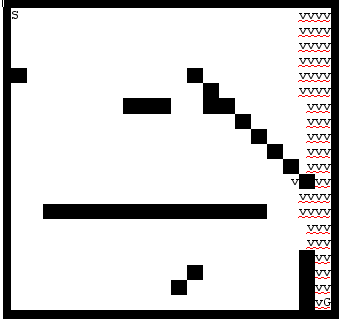
\includegraphics[scale=0.65]{visFromGoal.png}
\caption{A PPP with 8\% Goal visibility. 'v' symbols represent the squares from which the goal is visible to a perfect sensor.}
\label{fig:goal_vis_ppp}
\end{figure}

After prototyping a set of PPPs with this fitness function, I noted that the generator was encouraged to place obstacles in clusters around the goal position such that the greatest number of cells were obscured. Placing obstacles further away is less attractive, as it leaves many cells on the side of the goal which can still 'see' into the goal. As a result, chromosomes which produce obstacles further from the goal tend to be bred out over the course of the tournament. At the extreme, this resulted in PPPs which were mostly empty with the exception of these blocking obstacles, and thus were easy to traverse.

\subsection{Visibility Magnitude}
\label{sec:visMag}
To attempt to encourage the generator to spread obstacles across the PPP, I added additional measurements of visibility to the function. These measurements would take into account the visibility from each of the four corners and the centre of the PPP, in hope that the generator would be encouraged to spread the obstacles more evenly throughout the PPP. These five measurements would then be treated as a vector and the magnitude used as the final evaluation, acting as a measurement of the balance of visibilities from each position.

The fitness function was then tweaked to minimise this visibility; an example PPP produced under this function is provided in figure \ref{fig:vis_mag_ppp}.

\begin{figure}
\graphicspath{ {DesignImpPics/} }
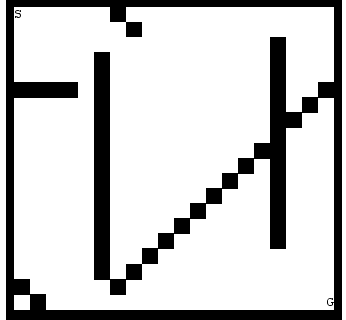
\includegraphics[scale=0.65]{visMag.png}
\caption{A PPP generated under Visibility Magnitude (Score=0.57).}
\label{fig:vis_mag_ppp}
\end{figure}

After prototyping a set of PPPs under this fitness function, I noted that many PPPs did indeed seem to spread obstacles more evenly across the environment. Furthermore, the additional viewpoints had forced the generator to make use of more of the budget of obstacles. 

However, the generator only protects the start and goal positions --- that is, it ensures these positions are never blocked by an obstacle. The other three measurement positions were not under this protection; hence, a large fitness reward could be received by simply placing a single obstacle on each of these positions. In the worst case, this resulted in PPPs with obstacles clustered tightly around the start and goal corners, with single obstacles on the other three measurement positions. In addition, given that five measurements made up the vector, it was not intuitive to identify a difficult PPP given the magnitudes alone. Furthermore, it was not clear how to add measurements of other features of the PPP to this vector. As a result, I decided it was not a sufficient description of a PPP's difficulty.

\subsection{Weighted Sum Function}
\label{sec:weighted_sum}
In order to address the issue of incorporating measurements of many features of a PPP into a single evaluation, I reworked the visibility magnitude function into a sum of visibilities. This would allow additional feature measurements to be added as terms to this function; a more intuitive description than the vector. Furthermore, terms of the function could be weighted to influence the generator to focus more or less on each feature. As noted, the visibility measurements would make up one feature of this function.

A particular flaw of the previous measurements I had implemented was that a PPP could receive a good score while using few obstacles. This left the PPP environment wide open, resulting in high pass rates that were not reflective of the score given to them by the fitness function. I therefore introduced a cost to using few obstacles to the weighted sum, hoping to encourage the generator to use more of the budget of obstacles given to a PPP producing a less open environment. This term is described as a percentage of the maximum obstacles per PPP, which is a configurable generator parameter.

With this basic function in place, I continued prototyping PPPs and investigating to identify good and bad features. This led me, for example, to weighting the start and goal visibilities more highly such that the generator considered them more important than the other viewpoints. An example of a PPP generated with these weights is presented in figure \ref{fig:weighted_sum_ppp}.

\begin{figure}
\graphicspath{ {DesignImpPics/} }
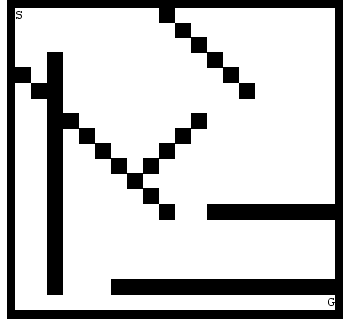
\includegraphics[scale=0.65]{goalStartVis.png}
\caption{A PPP with low start and goal position visibility.}
\label{fig:weighted_sum_ppp}
\end{figure}

In addition, I added new feature measurements to the function. I observed that many PPPs were generating with only one turn needed to reach the goal along the optimal path --- this meant that the path was the same as an empty PPP. See figure \ref{fig:one_turn_ppp} for an example of such a PPP. I therefore penalised PPPs with one turn in the fitness function. Furthermore, I noted that many PPPs with high pass rates across the agent set were often very open --- obstacles were clustered up or usage was low, such that much of the environment was wide 'plains' rather than a more maze-like structure. I therefore measured the maximum openness horizontally and vertically across each row and column --- that is, the maximum number of cells an agent could move in each without meeting an obstacle. I then averaged this across all rows and columns to produce a measurement of the average vertical and horizontal 'openness' of the PPP. Figure \ref{fig:open_ppp} shows an example PPP which is very open on both axes. I also experimented with other features, but removed them as the prototype results were worsened.

\begin{figure}
\graphicspath{ {DesignImpPics/} }
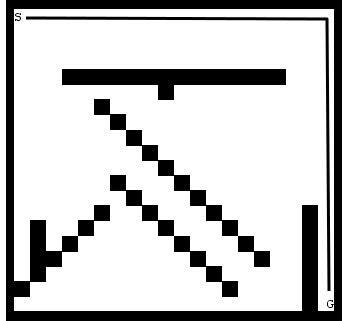
\includegraphics[scale=0.65]{oneTurn.png}
\caption{ A PPP with one turn on the optimal path, marked.}
\label{fig:one_turn_ppp}
\end{figure}

\begin{figure}
\graphicspath{ {DesignImpPics/} }
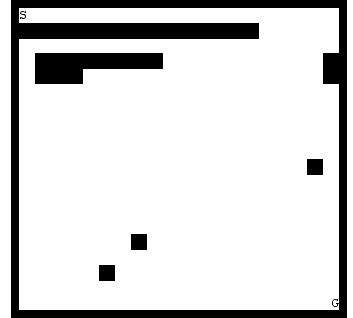
\includegraphics[scale=0.65]{wide_plain.png}
\caption{ A very open PPP.}
\label{fig:open_ppp}
\end{figure}

\subsection{Final Evaluation Function}
\label{sec:function}
After the tweaks, weights and additional measurements had been added, the fitness function was finalised into the form given in equation \ref{eq:fitness_func}. The generator seeks to minimise this function, a result of it being built initially upon the idea of minimising visibilities.

\begin{multline}
VisibilityFunction + 2\times(1-ObstacleUse)\\ + 2\times(AvgHorizonalOpenness) + 2\times(AvgVerticalOpenness)\\+ (2 \text{ if } OptimalTurns \equiv 1 \text{ else } 0))
\label{eq:fitness_func}
\end{multline}

Where 'VisibilityFunction' is the function given in equation  \ref{eq:vis_function}, denoting the weighted sum of the number of cells visible from each position named:
\begin{equation}
\resizebox{0.9\textwidth}{!}{$
1.5 \times \text{Start}+\text{Centre}+\text{Top Right}+\text{Bottom Left}+2.5 \times \text{Goal}
$}
\label{eq:vis_function}
\end{equation}

\section{Taxonomic Characters}
\label{sec:taxchar_design}
As described in section \ref{sec:da_7}, many new features of the environment of a PPP are now quantitatively evaluated as part of the process of difficulty evaluation. These features are stored individually as variables, and have been added to the existing taxonomic character classes to improve their ability to describe the environment.

Wei normalised his existing characters to a 0--1 range to ensure no taxonomic character dominated the others. Where necessary, this has been carried out.

Ashlock notes that further taxonomic characters might be derived from the behaviour of test agents on the PPP \cite[section 7B]{ashlock}. However, this would couple descriptions of PPPs to the agents expected to be simulated on them. As this project focuses on more general application of PPPs to autonomous agents, I have not added such characters. Instead, the characters added are geometric descriptions of the PPP extracted from obstacle layout --- for example, the characters describe the amount that these obstacles obscure the PPP from given viewpoints. Further work might describe the PPP using the descriptors of the PPP (for example, the number of diagonal descriptors) though Ashlock notes that these are generally less useful, being linked to the specific PPP representation\cite[section 7B]{ashlock}.

\section{Third Party Libraries}
\label{sec:tplibs}
The following third party libraries were used during the project.

\textbf{D3.js 3.5.16 \cite{d3js}}\\
A JavaScript library for manipulating documents based on data. This is used for visualisation of UPGMA tree structures, alongside a tree graph document produced by modifying an example graph.\\

\textbf{A* Path planning \cite{aStar}}\\
Pseudocode implementation of the A* algorithm, slightly modified to make use of the simulator data structures.\\

\textbf{Line Drawing on Grids \cite{lineDrawing}}\\
Implementation of Linear Interpolation and Line drawing on grids used to produce lines of sight by the agent's sensor components. As above, slightly modified to make use of simulator data structures.

\chapter{Evaluation}
\label{cha:Evaluation}
This chapter describes evaluation of the outcome of this project. First, I will discuss and evaluate the requirements stated in chapter \ref{cha:ProbAnalysis}. Following this, I will evaluate the improvements to the generator by testing the ability of the produced PPPs to discover faults and the diversity as described by the UPGMA graph.

\section{Analysis of Requirements}
\label{sec:req_eval}
This section focuses on the requirements stated in tables \ref{table:simreq} and \ref{table:genreq}. The requirements are evaluated to ensure they have been met.

\subsection{Simulator Requirements Evaluation}
\label{sec:sim_req_eval}
The simulator accepts and loads PPPs as produced by the generator in the .ppp format. These files are parsed and rebuilt using the existing PPP class such that the environment matches the PPP as displayed during generation and as recorded in the file. This satisfies requirement S01. 

Seven test agents, as described in chapter \ref{cha:Design} section \ref{sec:da_5}, have been produced. These agents range in capabilities, exhibiting different faults and approaches to path finding. Furthermore, all agents may be handicapped further with a limited memory and sensor noise. Thus, S02 has been met.

The simulation terminates when an agent reaches the goal position, or when a configurable move budget has been exhausted. This budget is set to 300, giving plenty of time for the agent to reach the goal if it is capable of doing so. Once all tests have terminated, the simulator produces a CSV file recording the details of PPPs and agents tested. S03 and S04 are therefore satisfied.

\subsection{Generator Requirements Evaluation}
\label{sec:gen_req_eval}
As described in chapter \ref{cha:Design} section \ref{sec:function}, an evaluation function has been produced assessing features of the PPP which relate to how difficult the environment is to explore. This function is reported in equation \ref{eq:fitness_func}. In addition, a fitness function has been added to the generator allowing it to select for difficulty during tournament generation of PPPs. Thus, R01 is satisfied. These functions may be adjusted, allowing the difficulty of PPPs to be produced --- for example, by reducing the weights in the function to produce more open PPPs. This satisfies R02.

The generator produces a variety of visually diverse PPPs with a range of success rates across the test agents satisfying R03. This will be discussed further in sections \ref{sec:gen_eval} and \ref{sec:div_eval}.

Finally, the features measured as part of the difficulty evaluation have been added as taxonomic characters and normalised as per the original characters. Thus, R04 and R04a have been satisfied.

\section{Evaluation of the Generator}
\label{sec:gen_eval}

In this section, I will evaluate the ability of the extensions made to the generator to find faults in the test agents. This will be compared to the original generator such that comparisons can be drawn.

\subsection{Methodology}
\label{sec:gen_eval_method}

The extensions to the generator were evaluated by producing a set of 60 PPPs using the new fitness function. In addition, a set of 60 PPPs was generated using Wei's "number of turns" fitness function. Both sets were generated via 10,000 mating events before being saved to disk.

The simulator I developed was used to test the ability of the generated PPPs to discover the faults in the test agents. Each agent was tested on each PPP 1,000 times and the percentage of passes --- when the agent reached the goal position --- recorded. This was to make the impact of non-determinism in the path planning algorithms, where tie-breaks occurred, negligible. In addition, various features of the PPP were recorded as evaluated by the generator functions. This data was written to a CSV file.

The test agents, as described in section \ref{sec:da_5} were used to evaluate these PPPs. For all agents, their sensor range was set to two --- that is, they could see two cells in all directions around them. Two Wallfollower agents were used, following walls to their left and right respectively. In addition, an explorer handicapped with a 5x5 limited memory and an explorer with a sensor noise of 0.1 were added, with the expectation that these agents would have lower pass rates in comparison to the unhandicapped explorer.

Example PPPs generated by both functions are presented in figure \ref{fig:wei_ppp} and \ref{fig:weighted_sum_ppp}.

\begin{figure}
\graphicspath{ {EvalPics/} }
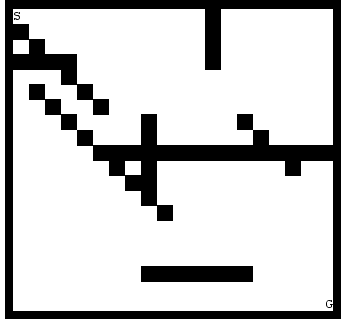
\includegraphics[scale=0.65]{wei_26.png}
\caption{PPP generated by Wei's function with 10 Turns}
\label{fig:wei_ppp}
\end{figure}

\begin{figure}
\graphicspath{ {EvalPics/} }
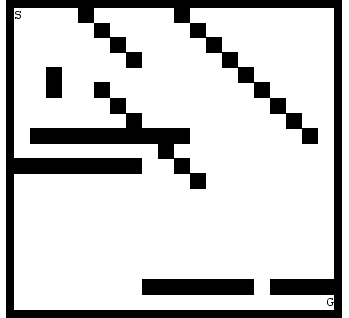
\includegraphics[scale=0.65]{openh_46.png}
\caption{PPP generated by the difficulty function}
\label{fig:difficulty_ppp}
\end{figure}

Finally, I compared the results on the set of Wei's maps against my own.

\subsection{Results}
\label{sec:gen_eval_results}

A full set of results for both PPPs generated with Wei's function and the my function are presented in appendix \ref{cha:gen_eval_appendix}.

The average pass rates across all 60 PPPs, for both Wei's and my PPPs, are presented in tables \ref{table:wei_eval} and \ref{table:diff_eval} respectively. Note that since the A* agent has perfect prior knowledge of the environment and always passes, it has been omitted. In addition, the random agent has been omitted as it is not particularly informative, being completely non-deterministic. The results for both omitted agents are available in the appendix \ref{cha:gen_eval_appendix}.
\begin{table}
\begin{tabular}{|l|l|l|l|l|l|l|l|l|}
\hline
Agent&WFL&WFR&Explorer&Exp.[5x5]&Exp.[Noise]&L.T.Exp.&Bumper&DBumper\\
\hline
Pass\%&74.5&78.33&76.82&16.55&65.93&97.01&32.19&32.86\\
\hline
\end{tabular}
\caption{Results for Wei's PPPs}
\label{table:wei_eval}
\end{table}

\begin{table}
\begin{tabular}{|l|l|l|l|l|l|l|l|l|}
\hline
Agent&WFL&WFR&Explorer&Exp.[5x5]&Exp.[Noise]&L.T.Exp.&Bumper&DBumper\\
\hline

Pass\%&81.24&93.33&80.90&18.84&68.15&94.82&71.12&73.45\\
\hline
\end{tabular}
\caption{Results for my PPPs}
\label{table:diff_eval}
\end{table}

As is clear from the tables, the results for the PPPs evolved under the difficulty function are worse, with the exception of the Long Term Explorer.

The results were compared statistically per agent using the Mann-Whitney test. Most agents were not significantly worse off. However, the following agents were saw statistically significantly poorer results over my PPPs. \\

The \textbf{Explorer with sensor noise} (z=2.3) with p=0.02.

The \textbf{Bumper} agent (z=5.6) and \textbf{Decision Bumper} agent (z=5.51), p$\approx$0.

\section{Evaluation of Diversity}
\label{sec:div_eval}
This section discusses the diversity of the produced PPPs, recalling that it is necessary that the produced test cases are diverse such that a wide range of environments are tested.

\subsection{Methodology}
\label{sec:div_eval_method}
In Ashlock and Wei's work, UPGMA is used to produce a tree structure describing the diversity of a set of PPPs. However, as noted in section \ref{sec:da_3_4}, the existing taxonomic characters --- turns, advances, (moves+turns) and obstacles, are not sufficient to describe PPPs clearly. It is often the case that this simple character set groups PPPs together because they have similar numbers of moves required to traverse them, though their layouts are wildly different. Therefore, additional characters were added.

Using the set of PPPs generated by Wei's fitness function in section \ref{sec:gen_eval_method} above, UPGMA trees will be produced with the original fitness function and the improved fitness function.

Since it has been shown in section \ref{sec:gen_eval_results} that the PPPs produced under the difficulty function are inferior in ability to find faults in the test agents, the diversity of these PPP environments will not be discussed.

\subsection{Results}
\label{sec:div_eval_res}
Figures \ref{fig:wei_tree} and \ref{fig:new_tree} reproduce UPGMA trees under Wei's taxonomy and the extended taxonomy, respectively. These trees are generated from the map sets discussed above.

\begin{figure}
\graphicspath{ {EvalPics/} }
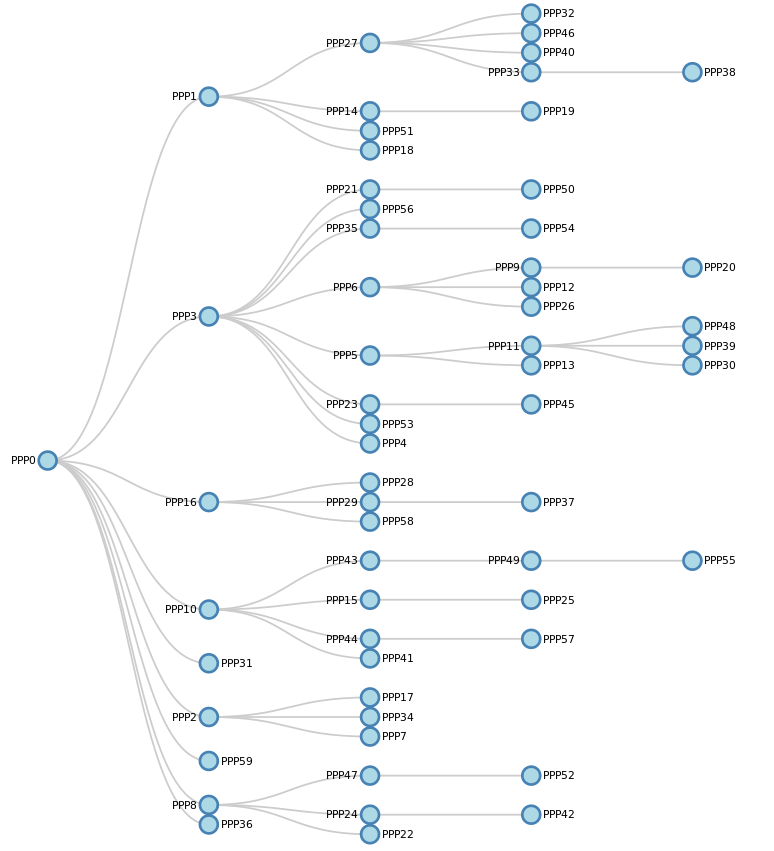
\includegraphics[scale=0.5]{wei_tree.png}
\caption{UPGMA tree for Wei's taxonomy.}
\label{fig:wei_tree}
\end{figure}

\begin{figure}
\graphicspath{ {EvalPics/} }
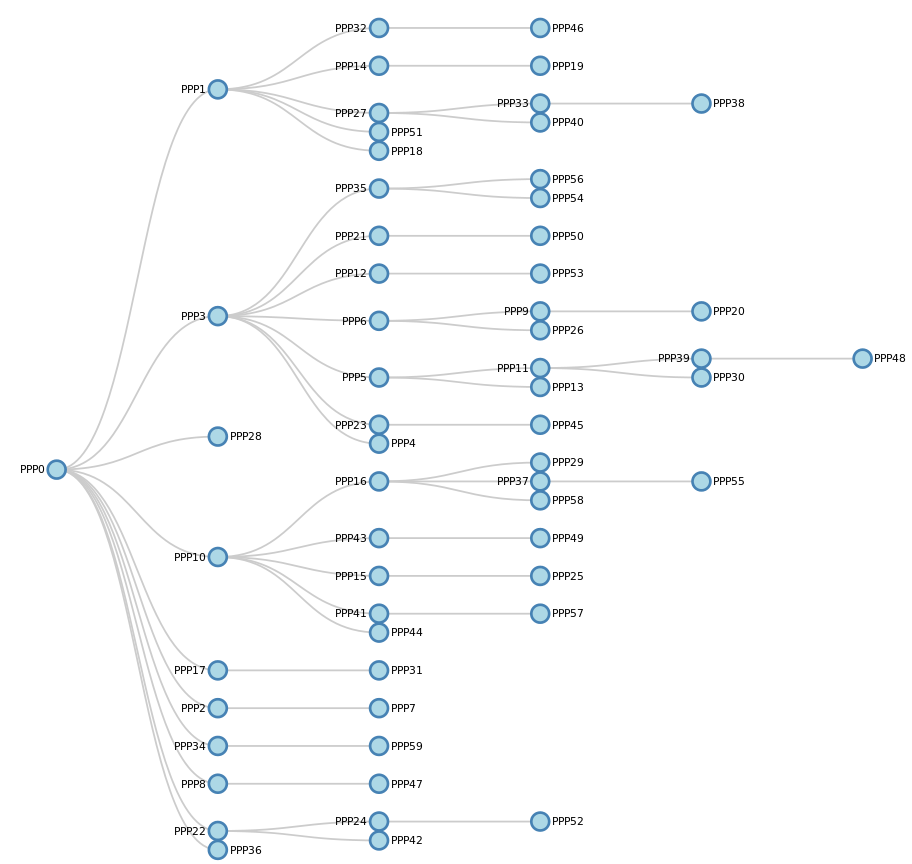
\includegraphics[scale=0.5]{new_tree.png}
\caption{UPGMA tree for extended taxonomy.}
\label{fig:new_tree}
\end{figure}

It can be seen that the tree in the extended taxonomy is deeper, suggesting further specialisation of the PPPs within the groups. It should be noted, however, that tree selection methods in biology often prefer trees that minimise total depth \cite[chapter 11 p.415]{phylo}. With this in mind, it is important to note that although the new taxonomy has a branch which is deeper than Wei's taxonomy, it also produces more group branches with shallow depths.

Finally, let us briefly consider the grouping of PPPs between the two trees. Consider the top branch in figure \ref{fig:wei_tree}, grouping PPPs 32, 33, 40, and 46 under PPP27. Several PPPs in this grouping have very different layouts; consider PPPs 27 and 46 in figures \ref{fig:ppp_27} and \ref{fig:ppp_46}. It can be seen that PPP27 requires less turns and moves, is less open, and concentrates less obstacles in the top left of the environment.

\begin{figure}[H]
\graphicspath{ {EvalPics/} }
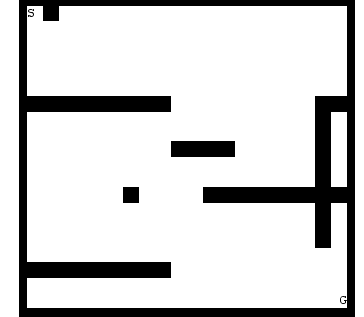
\includegraphics[scale=0.65]{ppp27.png}
\caption{PPP27, grouped with PPP46 via Wei's taxonomy.}
\label{fig:ppp_27}
\end{figure}

\begin{figure}[H]
\graphicspath{ {EvalPics/} }
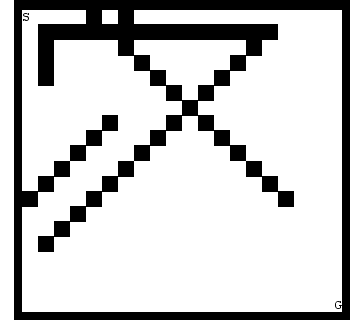
\includegraphics[scale=0.65]{ppp46.png}
\caption{PPP46, grouped with PPP27 via Wei's taxonomy.}
\label{fig:ppp_46}
\end{figure}

In the extended taxonomy tree, PPP46 is instead grouped with PPP32 (see figure \ref{fig:ppp_32}). These PPPs have more similar layouts, with a high number of turns and a concentration of obstacles in the top half of the map. This suggests the extended taxonomy better classifies the PPPs.

\begin{figure}[H]
\graphicspath{ {EvalPics/} }
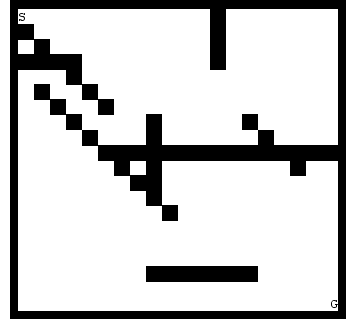
\includegraphics[scale=0.65]{ppp32.png}
\caption{PPP32, grouped with PPP46 via the extended taxonomy.}
\label{fig:ppp_32}
\end{figure}


\part{Closing Remarks}
\label{sec:close}
\chapter{Conclusion}
\label{cha:conclusion}
\subsection{Fault finding}
\label{sec:conc_fault}
It is clear from the evaluation in section \ref{sec:gen_eval_results} that the test agents saw higher pass rates across the board on my PPPs, with three agents seeing pass rates that were higher with statistical significance. As a result, it is clear that this approach to generating PPPs does not improve the ability to find faults in test agents.

Despite this, the evaluation of various features of the PPPs has produced a set of valuable taxonomic characters, as discussed below. Therefore it can be said that although the fault finding has not been improved, the introduction of difficulty into PPP evaluation has not been without value.

Furthermore, it should be noted that this project focused only on one specific factor of difficulty --- the degree to which the PPP environment is difficult to explore --- and that many more were identified in the literature review. Not all of these are directly applicable to the very simplistic PPP environment currently generated, however --- for example, with a singular agent and goal, it is not necessary to coordinate a team or prioritise objectives such as the challenges in RoboCup. However, other factors are easily implementable or modifiable such that they could be represented. For example, terrain types with different movement costs could be included, and a more sophisticated sensor model used to represent agents with restricted fields of view and multiple sensors.

As such, there may be value in considering alternative measurements and factors of difficulty in the future.

\subsection{Diversity}
\label{sec:conc_div}

As discussed in section \ref{sec:div_eval}, new taxonomic characters have been produced, based on measurements obtained during the difficulty evaluation stage of PPP generation. These have been used to extend the neighbour joining taxonomy, offering a greatly improved description of the PPPs produced by the generator.

This has resulted in a better classification of the PPPs into groups via the UPGMA algorithm. The richer description of PPPs produces groups wherein the layouts are much more similar. In addition, it is now more common to see PPPs grouped together with distinguishing features; for example, PPPs which cluster obstacles heavily in a quadrant or half of the map now tend to be grouped together. Under the original taxonomy, it was the case that PPPs often had very different layouts but were grouped together because they had, for example, a similar number of turns required on the optimal path.

By better classifying the PPPs, in particular by producing groups with more similar layouts, it is now possible to more easily select a wide range of diverse PPPs for testing by selecting PPPs from several branches of the tree. Under the original taxonomy, this would also have required the user to visually inspect the PPPs to ensure the layouts were in fact varied enough, a time consuming task. Furthermore, this improved classification opens the path to allow automatic suggestion of PPPs to be used based on the taxonomy. For example, if 10 PPPs were requested, the generator could classify the set of PPPs and then select the PPPs from as many distinct groupings as possible.

The result of this is that, although this project has not resulted in increased fault finding capability in the PPP environments themselves, it should be possible to improve fault finding via the improved ability to select diverse PPPs from the existing generation methods, using evaluations produced by this project.

\chapter{Future Work}
\label{cha:futWork}
As discussed in the literature review, there are numerous factors of difficulty which could be considered to continue this line of work. However, due to the simplistic nature of the current PPPs, it is likely the case that many of these factors would not be easily applicable. Therefore, I would suggest that the PPP environment is first extended if further evaluations are to be considered. For example, additional terrain types could be added with increased movement costs. Given the simplicity of the current PPPs, it is possible that there is little to be gained via further evaluations over simple factors such as Wei's existing functions.

In addition, I would suggest that focus is placed more on the diversity of PPPs produced by the generator. For example, modification could be made to the generator to produce a large number of PPPs, 'banking' them over time and switching to other fitness functions with the remainder. This would result in a diverse range of PPPs wherein each subset would have been produced by different fitness functions.

Furthermore, it is still difficult to deduce the diversity of the produced set of PPPs via UPGMA alone, often requiring manual observation to be made. While this has been improved by the new taxonomic characters, it is still unclear what the diversity of the entire group of PPPs is from the tree alone. Optimality criteria for these neighbour trees might be implemented, such as those described in \cite[chapter 11, p.~426]{phylo}, to better explain this. Furthermore, methods for comparison of two trees \cite[chapter 11 p.~504]{phylo} might be implemented to assist in drawing large sets of test PPPs from multiple generator runs; perhaps produced via different fitness functions.

\begin{thebibliography}{56}
\bibitem{umerson}
	C. Umerson et al.,
	"Autonomous Driving in Urban Environments: Boss and the Urban Challenge",
	J. Field Robotics Special Issue on the 2007 DARPA Urban Challenge,
	vol. 1 no. 8 pp.~425-466
	Jun. 2008
	
\bibitem{guizzo}
	E. Guizzo.
	(2011, Oct. 18).
	How Googles Self Driving Car Works [Online].
	Available: http://spectrum.IEEE.org/automaton/robotics/artificial-intelligence/how-google-self-driving-car-works, 
	
\bibitem{rob}
	R. Alexander et al.,
	"Situation coverage - a coverage criterion for testing autonomous robots",
	Dept. Computer Science, University of York,
	Report Number YCS-2015-496,
	Apr. 2015
	
\bibitem{ashlock}
	D. A. Ashlock et al.,
	"Evolving A Diverse Collection of Robot Path Planning Problems" in
	IEEE Congress on Evolutionary Computation,
	Vancouver, BC
    2006, pp.~1837 - 1844 

\bibitem{wei}
	H. Wei,
	"Evolving path-planning problems to find faults in autonomous mobile robots",
	MSc thesis,
	Dept. Computer Science, University of York, York, N.Yorkshire, 2013

\bibitem{robocup}
	H.Kitano, S. Tadokoro,
	"RoboCup Rescue: A Grand Challenge for Multiagent and Intelligent Systems",
	AI Magazine,
	Vol. 22 No. 1, pp.~39-52,
	Spring 2001

\bibitem{jacoff}
	A. Jacoff et al.,
	"Performance Evaluation of Autonomous Mobile Robotics",
	Int. J. Industrial Robot,
	Vol. 29, No. 3, pp.~256-267,
	2002

\bibitem{maze}
	D.A. Ashlock et al.,
	emph{"Search-based Procedural Generation of Maze-Like levels"},
	IEEE. Trans. Comput. Intelligence and AI in Games,
	Vol. 3, No. 3, pp~260-273,
	Sept. 2011
	
\bibitem{jacoffGuide}
	Standard Test Methods for Response Robots, 
	ASTM International Standards Committee on Homeland Security Applications (E54.08.01),
	2015
	
\bibitem{meyer}
	J. Meyer, D. Filliat,
	"Map-based navigation in mobile robots:: II. A review of map-learning and path-	planning strategies",
	Cognitive Systems Research,
	Vol. 4 no. 4, pp.~283-317
	Dec. 2003
	
\bibitem{elfes}
	A. Elfes,
	"Using Occupancy Grids for Mobile Robot Perception and Navigation"
	Computer, 
	Vol. 22, no. 6, pp. 46–57, 
	Jun. 1989.
	
\bibitem{thrun}
	S. Thrun,
	"Learning Occupancy Grid Maps with Forward Sensor Models",
	Autonomous Robots,
	Vol. 15 no.2, pp.~111–127,
	Sept. 2003
	
\bibitem{lee}
	The Map Building and Exploration Strategies of a Simple Sonar-Equipped Mobile Robot
	D. Lee
	Cambridge University Press, 1996
	
\bibitem{slam}
	H. Durrant-Whyte, T. Bailey,
	"Simultaneous Localization and Mapping: part 1",
	IEEE Robot. Automat. Mag.,
	Vol. 13, No. 2, pp.~99-110,
	Jun. 2006
	
\bibitem{stentz}
	A. Stentz,
	"Optimal and Efficient Path Planning for Partially-Known Environments",
	Proc. IEEE Robotics and Automation,
	San Diego, CA,
	May 1994
	
\bibitem{d3js}
	M. Bostock,
	D3.js 3.5.16,
	Available: https://d3js.org/

\bibitem{aStar}
	A. Patel,
	A* Implementation Notes [Online]
	Available: http://theory.stanford.edu/~amitp/GameProgramming/ImplementationNotes.html

\bibitem{lineDrawing}
	Red Blob Games,
	Line Drawing on Grids [Online].
	Available: http://www.redblobgames.com/grids/line-drawing.html
	
\bibitem{agile}
	K. Beck et al.,
	(2001, Feb.)
	Agile Manifesto [Online].
	Available: http://agilemanifesto.org/
	
\bibitem{spiral}
	B. W. Boehm
	"A spiral model of software development and enhancement"
	Computer, 
	Vol. 21, no. 5, pp. 61-72, 
	May 1988.
	
\bibitem{phylo}
	D. L. Swofford et al.,
	"Phylogenetic Inference", in Molecular Systematics,
	2nd ed, Sunderland, MA., 1996, cha. 11, pp. 407-514

\end{thebibliography}

\begin{appendices}
\chapter{Appendix A: Generator Evaluation Results}
\label{cha:gen_eval_appendix}

\begin{table}[H]
\scriptsize
\begin{tabular}{|l|c|c|c|c|c|c|c|c|c|c|}
\hline
PPP	& A* & Random & WFL & WFR & Explorer& Explorer[5x5] & Explorer[noise] & LongTerm & Bumper & DBumper \\
\hline
PPP0&100&2&100&100&87.3&8.7&65.3&100&32.2&38.9\\
PPP1&100&0&0&100&28.8&11.4&25.6&74.5&0&0\\
PPP2&100&3.6&100&100&83.5&25.1&71.2&97.2&42.1&39.2\\
PPP3&100&2&100&100&76.8&18.3&66.7&100&67.2&74.6\\
PPP4&100&0.8&100&100&87.8&9.9&58&99.9&0&0\\
PPP5&100&5.2&0&0&70.5&19.2&72.7&99.4&75.4&84.6\\
PPP6&100&2.1&100&100&83&17.7&65.5&99.2&41.9&39.2\\
PPP7&100&1.8&100&100&88.8&5.6&65.2&100&0&0\\
PPP8&100&2.6&0&0&73.6&27.2&63.1&100&0&0\\
PPP9&100&0&50.8&100&73.2&36.4&63.5&98.6&0&0\\
PPP10&100&4.3&100&0&97.1&49.8&79.1&100&95.7&98.2\\
PPP11&100&2.7&0&100&82.1&11.4&77&100&0&0\\
PPP12&100&6.7&0&0&82.6&15&71.6&99.8&35.9&28\\
PPP13&100&2.5&100&100&96.2&18&75.7&100&70.5&66.7\\
PPP14&100&0.3&100&100&69.3&28&74.7&100&0&0\\
PPP15&100&3.1&100&100&93.1&18&76.9&100&63.4&56.6\\
PPP16&100&1&100&100&66.5&12.3&65.1&100&23.1&16.2\\
PPP17&100&3&0&0&60.6&9.1&50.5&97.9&0&0\\
PPP18&100&0&0&100&35.2&14.2&43.7&100&0&0\\
PPP19&100&0.8&100&100&49&4.3&32&22.2&0&0\\
PPP20&100&0&71.6&100&72&5.6&41.8&97.1&0&0\\
PPP21&100&3.6&100&100&98.3&29.4&86.9&100&96.6&100\\
PPP22&100&4.1&100&0&85.9&43.6&74.9&95.8&79&78.2\\
PPP23&100&3.7&100&0&94.6&33.4&81.4&100&94.2&96.4\\
PPP24&100&1.5&0&100&83.2&9.2&65.2&100&51.8&49.3\\
PPP25&100&3.3&100&0&94.2&9.2&73.5&100&80.8&86.1\\
PPP26&100&4.8&100&0&64.7&17.6&79&97&0&0\\
PPP27&100&0.2&100&100&82.6&7.5&62.8&93.6&0&0\\
PPP28&100&1.8&100&100&66.7&2.9&64.8&100&0&0\\
PPP29&100&2.3&0&100&97.1&9.2&69.8&100&52.3&52.3\\
PPP30&100&2.4&100&100&66.3&20.7&60.1&99.1&51.3&34.9\\
PPP31&100&1.9&0&0&87.5&14.5&79.7&100&0&0\\
PPP32&100&0.1&0&0&67&8.9&36.6&76.3&0&0\\
PPP33&100&1.7&100&100&64.8&11.1&58.1&99.9&33.7&34.8\\
PPP34&100&0&74.5&100&70.3&15.7&67.7&97.6&40.6&38.4\\
PPP35&100&4.9&100&0&79.5&10.6&71.6&99&38.8&40.6\\
PPP36&100&2.6&100&100&77.4&10.7&63.8&99.8&0&0\\
PPP37&100&2.1&100&100&91.9&22.6&71.5&96.3&54.5&51\\
PPP38&100&0&100&100&82&9.8&66&98.5&0&0\\
PPP39&100&2.4&100&100&68.4&4.9&68.4&99.5&0&0\\
PPP40&100&0&0&0&80.1&4.6&49.8&95.7&0&0\\
PPP41&100&2.2&100&100&72.9&27.9&73.1&99.2&0&0\\
PPP42&100&1.9&100&100&75.7&19.6&61.9&99.9&49.1&55.8\\
PPP43&100&2.9&100&100&85.7&16.2&75.9&100&94.8&100\\
PPP44&100&2.6&100&100&96&8.2&73.5&100&0&0\\
PPP45&100&2.3&100&100&55.2&12.9&66.1&100&0&0\\
PPP46&100&0&0&100&89.8&17.9&62&100&0&0\\
PPP47&100&2.3&100&100&46.5&2.9&58&97.5&0&0\\
PPP48&100&1.4&100&100&60.1&15.5&64.2&99.8&0&0\\
PPP49&100&2.6&100&100&83.2&26.6&77.7&100&71.9&73.9\\
PPP50&100&4.7&100&100&78.1&17.3&73.4&100&77&91.7\\
PPP51&100&0.2&0&100&74&19.4&68.5&98&63.9&70.1\\
PPP52&100&1.9&100&100&86.7&28.7&69.4&100&64.7&64.4\\
PPP53&100&3.3&100&100&93.4&13.1&74&95.6&0&0\\
PPP54&100&3.3&100&100&83.1&23.2&78.6&100&71.6&79.1\\
PPP55&100&2.3&100&100&80.8&14.4&63.2&100&65.7&74.5\\
PPP56&100&0&73.1&100&71&23.4&65.6&99.8&0&0\\
PPP57&100&1.9&100&100&97.1&23.9&81.1&100&83.4&82.4\\
PPP58&100&2.2&100&100&57.9&4.9&57.8&97.1&0&0\\
PPP59&100&3.2&100&100&62.3&15.5&55.1&99.8&68.5&75.5\\
\hline
\end{tabular}
\caption{Simulation Results for Wei's PPPs}
\end{table}

\begin{table}
\scriptsize
\begin{tabular}{|l|c|c|c|c|c|c|c|c|c|c|}
\hline
PPP	& A* & Random & WFL & WFR & Explorer& Explorer[5x5] & Explorer[noise] & LongTerm & Bumper & DBumper \\
\hline
PPP0&100&0.6&100&100&39.4&15.5&38.4&78.4&0&0\\
PPP1&100&2.9&100&100&95.2&31.7&78.4&97.2&99&99.6\\
PPP2&100&3.7&100&100&91.2&22.4&79.1&99.6&97.7&99.4\\
PPP3&100&3.4&100&100&90.4&11.8&82.1&99.2&84&92\\
PPP4&100&3.2&0&100&73.7&8.4&68.9&100&94.1&94.9\\
PPP5&100&3.2&100&100&62.6&15.6&66&96.9&0&0\\
PPP6&100&3.4&100&100&66&7.2&62.8&98.8&86.7&93.5\\
PPP7&100&3.8&100&100&86.9&12.1&76.8&100&75.5&93.3\\
PPP8&100&4&100&100&75&3.5&71&98.8&88.4&95.9\\
PPP9&100&1.7&100&100&82.6&10.8&69.6&99.9&0&0\\
PPP10&100&1&0&100&97.6&24&73.3&100&98.2&99.8\\
PPP11&100&1.4&100&100&70.8&13.5&69.5&99.8&0&0\\
PPP12&100&2.2&100&100&87.4&50.1&62&79&99.2&100\\
PPP13&100&3.2&100&100&73&17.9&74.7&100&38.1&31.3\\
PPP14&100&3.2&100&100&99.8&15.2&83&100&97.1&100\\
PPP15&100&3.8&100&100&84.4&15.3&76.6&97.6&97.2&99\\
PPP16&100&1.7&100&100&94.3&46.7&59.2&71.7&75.9&86\\
PPP17&100&2.2&100&100&74.2&28.6&70.1&99.8&81&86.4\\
PPP18&100&2.8&100&100&81.2&16.5&74.7&99.8&38.8&34.8\\
PPP19&100&0&76.3&100&44.7&10.2&24.6&89.5&64.3&62.4\\
PPP20&100&2.1&100&99.9&67.2&11.1&60.6&99.1&55.3&45.7\\
PPP21&100&0&43.4&100&83.4&3.1&20.3&95.2&99.7&100\\
PPP22&100&2.8&99.3&100&83.4&32.8&69.9&98.4&71.6&70\\
PPP23&100&0&78.5&100&89.3&20.4&66.4&99.9&50.1&44.1\\
PPP24&100&0&81.4&100&87.1&14&75.1&99.8&93.6&99.8\\
PPP25&100&1.6&0&100&94.5&29&79.8&99.9&99.4&100\\
PPP26&100&1&100&100&55.7&16.2&64.8&97.6&0&0\\
PPP27&100&0&49.7&100&70.5&14.9&27.4&23.1&73.4&74.3\\
PPP28&100&1.8&100&100&92.7&10.5&70.9&96.4&0&0\\
PPP29&100&0.8&0&100&57.7&15&33.1&99.7&62.8&65.2\\
PPP30&100&3.1&100&100&84.6&17.8&74&99.9&96.8&100\\
PPP31&100&4.2&100&100&95.5&26.6&83.5&100&94.3&98\\
PPP32&100&2.4&100&100&92.8&18.4&78&99.6&97.2&100\\
PPP33&100&3.1&100&100&92.4&34.9&81.9&100&97.4&99.6\\
PPP34&100&2.8&100&100&96.3&18&90.6&100&80.5&78.2\\
PPP35&100&4.1&0&100&95&30.1&78&100&96.3&98.8\\
PPP36&100&4.2&100&100&92.4&30.1&79.7&100&87.4&96.6\\
PPP37&100&2.1&100&100&86.8&37.4&75.5&100&98.7&100\\
PPP38&100&3.4&100&100&96.7&14.4&83.5&100&96.5&100\\
PPP39&100&0&88.6&100&83.9&17.8&64.1&98.7&80.9&90.9\\
PPP40&100&0.2&100&0&51.2&12.9&37.6&96.6&0&0\\
PPP41&100&0.5&100&99.6&56.3&7.2&52.7&83.4&93&96.4\\
PPP42&100&3.2&100&0&78.7&11.9&75.5&93.1&45.5&40.4\\
PPP43&100&3.1&0&100&93.4&23.5&84.2&100&62.9&62.1\\
PPP44&100&4.4&100&100&89.9&17.5&80.5&100&94.4&100\\
PPP45&100&3.3&100&100&72.7&12.8&71.9&99.7&89.8&95.6\\
PPP46&100&0&48.4&0&28.6&14.4&19.6&41.1&51.6&66.3\\
PPP47&100&2.2&0&100&93.1&29.7&79.1&99.9&100&100\\
PPP48&100&4.1&100&100&78.9&4.7&72.8&100&94.1&99.8\\
PPP49&100&1.6&100&100&69&2.6&45.9&80.2&0&0\\
PPP50&100&2.2&0&100&77.4&24&73.3&95.6&97.1&99.3\\
PPP51&100&0&74&100&78.6&28.6&70.5&99.5&78.8&84.5\\
PPP52&100&2.2&100&100&99.8&21.3&78.9&100&24.5&19.9\\
PPP53&100&2.5&100&100&91.7&17.2&75.4&95.1&91.9&95.9\\
PPP54&100&2.8&100&100&97.1&16&77.2&100&79.2&92.1\\
PPP55&100&1.6&99.5&100&92.9&20.3&83.8&100&97.8&100\\
PPP56&100&3.4&100&100&86.1&18.2&80.1&99.7&89.7&84.7\\
PPP57&100&0&48.8&0&72.7&9.4&63.1&93&47.9&46.6\\
PPP58&100&0&86.7&100&82.1&27.7&69.1&98.9&83&94\\
PPP59&100&2.5&100&100&95.7&21&80&100&98.8&100\\
\hline
\end{tabular}
\caption{Simulation Results for My PPPs}
\end{table}

\end{appendices}

\end{document}
